% !TEX root = ../main.tex
%
\chapter{User Interface Design}
\label{sec:design}

This chapter outlines the design of the prototype, focusing in the user interface and the user experience. The design process was informed by the initial user research.

\section{User Flow and Navigation}
\label{sec:design:flow}

As an initial step in the design process, a user flow diagram was created to visualize required user interaction and their relations. 
In a first rough sketch, key interactions were arranged in a linear sequence, representing the typical workflow when creating NeRF models (\ref{fig:design:flow-1}).

\begin{figure}[htb]
	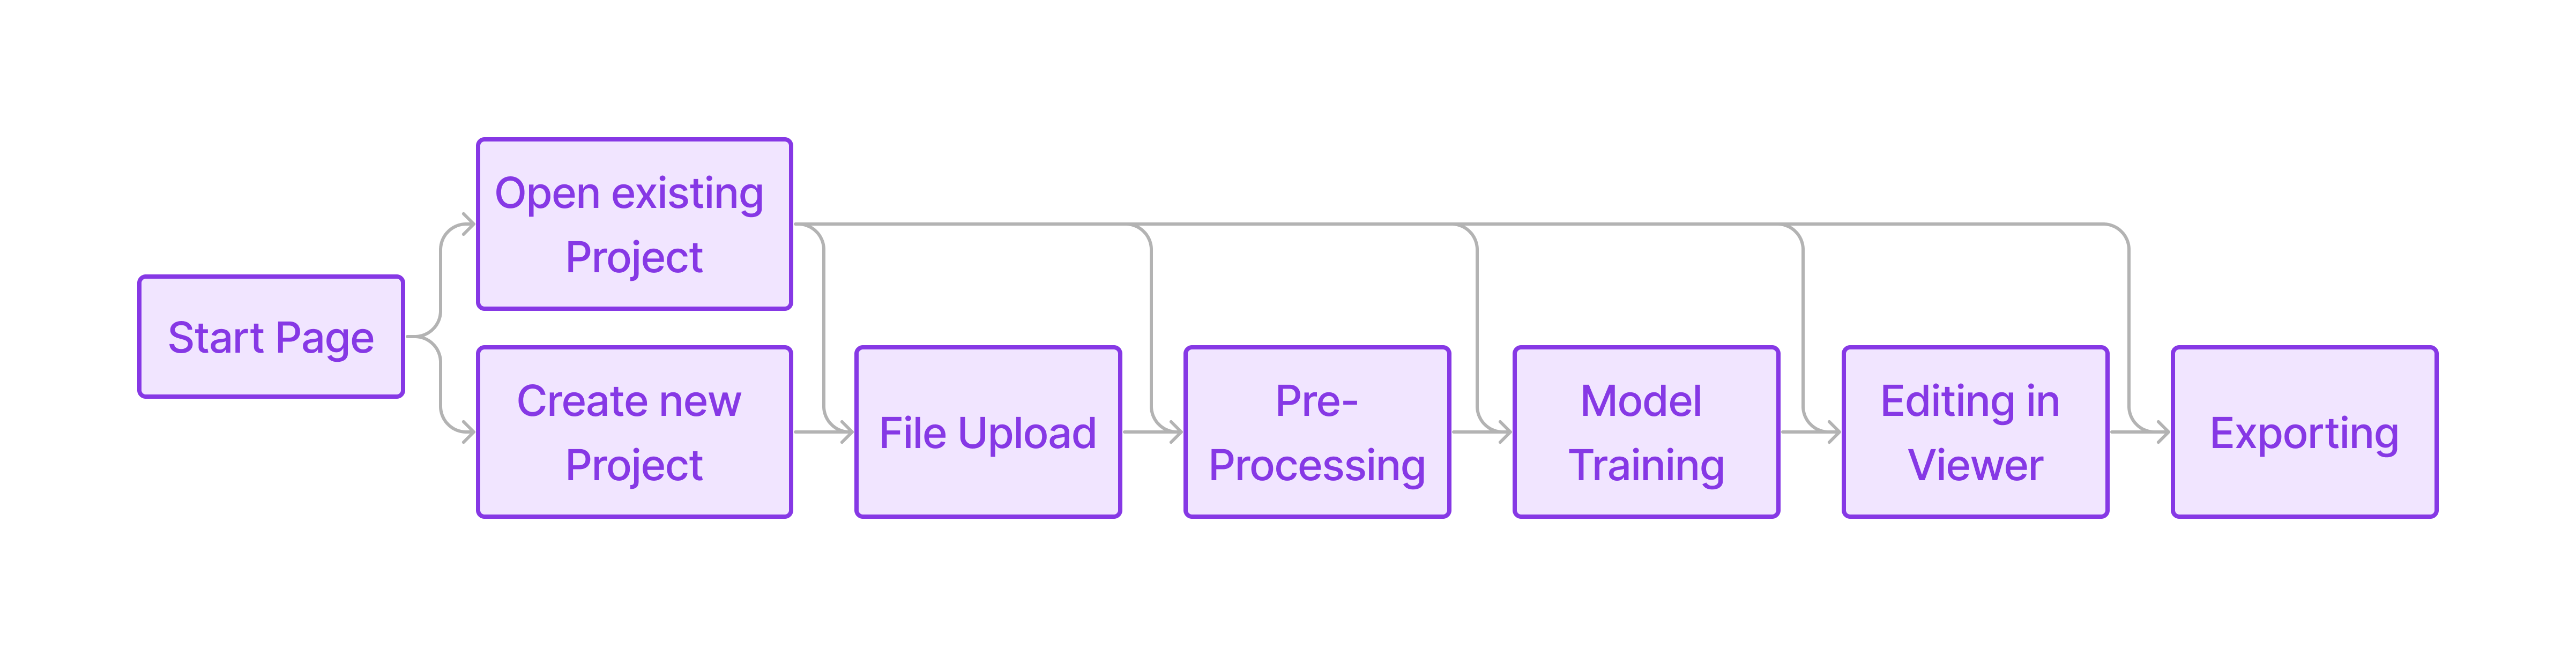
\includegraphics[width=\textwidth]{figures/flow-1.png}
	\caption{Flow Diagram}
	\label{fig:design:flow-1}
\end{figure}

Building on this outline, complex interaction were broken down into smaller steps to scope out what user actions were required to complete a task.
Interactions could then be group into views, and the navigation between these views could defined.
The views were also enriched with more detailed information on the exact user interactions (\ref{fig:design:flow-2}).

\begin{figure}[htb]
  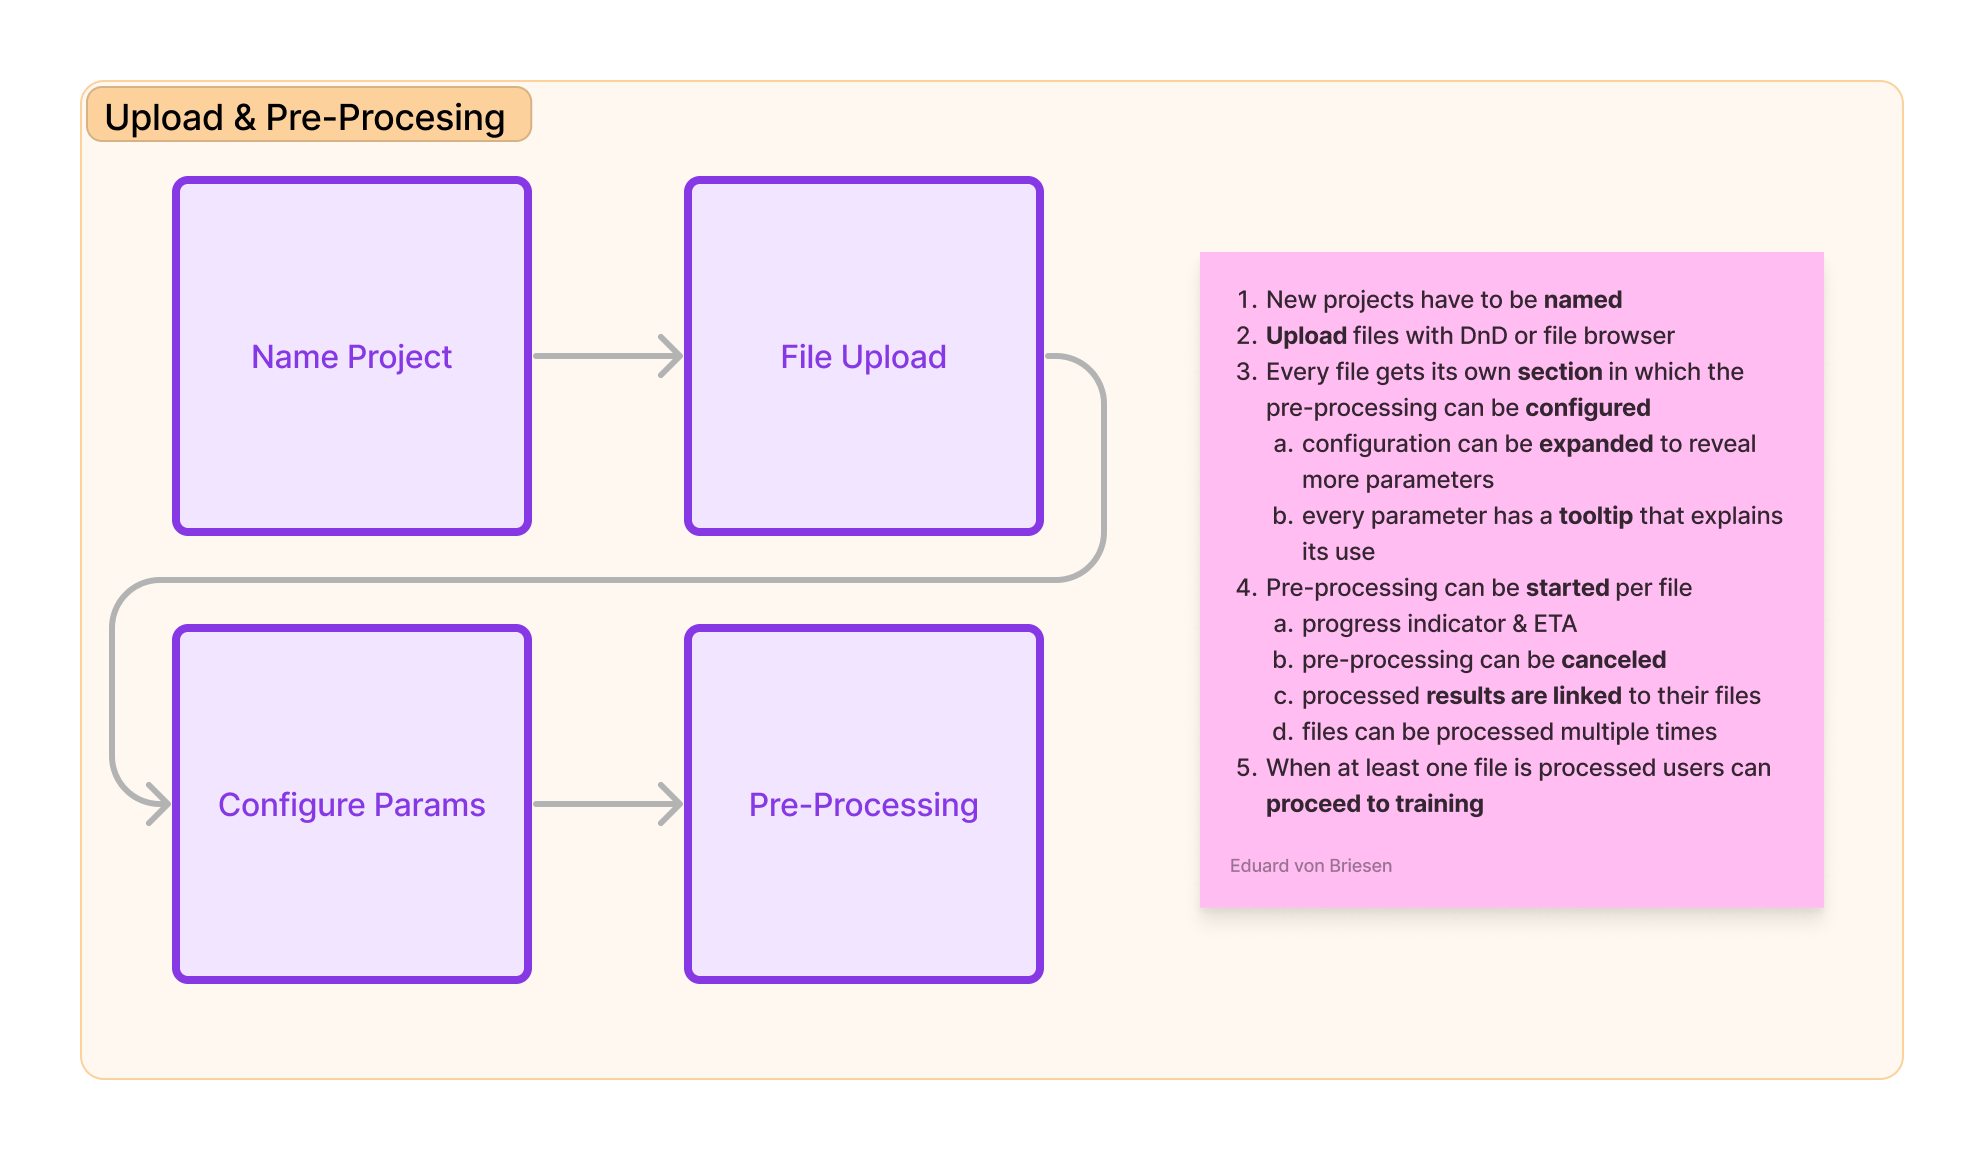
\includegraphics[width=\textwidth]{figures/flow-2.png}
  \caption{Excerpt of a View from the Flow Diagram with detailed interactions}
  \label{fig:design:flow-2}
\end{figure}

These diagrams were used as a reference throughout the design and development process, to ensure a structure that followed the user's mental model and to keep the user interface consistent.

\section{User Interface}

\subsection{Dashboard}

\subsection{Configuration}

\subsection{Model Editing}